\documentclass[11pt,a4paper]{article}
\usepackage[T1]{fontenc}
\usepackage[utf8]{inputenc}
\usepackage[english]{babel}
\usepackage{lmodern}
\usepackage[margin=2.2cm]{geometry}
\usepackage{amsmath,graphicx,booktabs,xcolor,caption}
\usepackage{pgfplots}
\pgfplotsset{compat=1.16}
\usepackage[hidelinks]{hyperref}
\setlength{\parindent}{0pt}\setlength{\parskip}{6pt}

\definecolor{frozen}{HTML}{1552AD}
\definecolor{full}{HTML}{C13B21}
\newcommand{\src}{../../../../reports/experiments/experiment_81_execution_20261106/figures}
\newcommand{\reading}[1]{\textbf{Reading.} #1}

% The four curves of one quantity: colour = arm, line style = video set.
\newcommand{\four}[1]{%
  \addplot[frozen,thick] table[x=update,y=#1]{frozen_train.dat};
  \addplot[frozen,thick,densely dashed] table[x=update,y=#1]{frozen_selection.dat};
  \addplot[full,thick] table[x=update,y=#1]{full_train.dat};
  \addplot[full,thick,densely dashed] table[x=update,y=#1]{full_selection.dat};}
\pgfplotsset{curve/.style={width=\linewidth,height=5.3cm,xmin=0,xmax=100,
  xlabel={Optimizer update},grid=major,grid style={gray!20},
  extra x ticks={20.5},extra x tick labels={},extra x tick style={grid=major,grid style={black!60,densely dotted,thick}},
  tick label style={font=\footnotesize},label style={font=\footnotesize},title style={font=\small\bfseries}}}

\begin{document}

{\LARGE\bfseries Experiment 81: reading the figures}\\[2pt]
{\small Document of 10 November 2026. No training was rerun for this document.}

\section*{What was trained}

80 thermal videos: 40 without a spill (\emph{clean}) and 40 with a spill (\emph{cold}).
64 are used for training and 16 for selection. Two versions of the same model are compared,
with the same videos, the same seed (239) and 100 updates each:

\begin{itemize}\itemsep1pt
\item \textcolor{frozen}{\textbf{frozen} (blue)}: the pretrained V-JEPA~2 video encoder stays fixed; only the small temporal module is trained.
\item \textcolor{full}{\textbf{full} (red)}: the 24 blocks of the encoder are trained as well.
\end{itemize}

The loss is the sum of four terms:
\[
L \;=\; L_{\text{ViCo}} \;+\; 0.1\,L_{\text{align}} \;+\; L_{\text{predict}} \;+\; 0.1\,L_{\text{keep}} .
\]

In every curve: solid line = training videos, dashed line = selection videos.
The dotted vertical line marks the end of the 20-update curriculum; the state of the AdamW
optimizer is reset before update 21, as the protocol specifies.

\textbf{About the redrawn curves.} Figures 2 and 3 are redrawn from the recorded values,
with no smoothing and no change to any value. Only the presentation changes: graduated axes,
a legend, and a logarithmic scale where a curve spans several orders of magnitude. The original
figures are reproduced in the annex.

\textbf{A limit to keep in mind.} The 16 selection videos come from the same recording
conditions as the training videos and have been used for many checks. They are not an
independent test set.

\newpage
\section*{Figure 1: t-SNE before any training}

\begin{center}\includegraphics[width=.8\linewidth]{\src/tsne_frozen_initial.png}\end{center}

\textbf{What is plotted.} Each point is one video, represented by the 128-dimensional vector
the model produces at update 0, that is, before any learning. t-SNE projects these 80 vectors
into two dimensions while keeping similar videos close together.
Blue = no spill, red = spill; circle = training (64), square = selection (16).

\textbf{What we observe.}
\begin{itemize}\itemsep1pt
\item The blue and red points form two disjoint groups; no point of one class lies inside
      the group of the other.
\item A small isolated blue group on the left contains 7 videos: \texttt{videoFrame} 1, 3, 4, 5, 6, 7 and 8.
\item At this same update 0, all 16 selection videos are already classified correctly, and
      63 of the 64 training videos.
\end{itemize}

\reading{The two classes are separated before the model has learned anything. The separation
therefore does not come from the loss. It is already in the videos themselves: the videos of the
two classes were recorded under different conditions (384$\times$288 for one class,
640$\times$480 for the other, different scenes). This explanation is an inference: the figure
shows that the separation exists beforehand, not what causes it.}

\textbf{What the figure does not show.} The axes of a t-SNE and the distances between its groups
have no meaning, and two t-SNE plots cannot be compared with each other. The figure says nothing
about where in the image the model looks.

\newpage
\section*{Figure 2: the terms of the loss}

\begin{center}
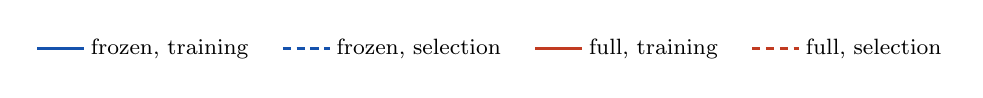
\begin{tikzpicture}
\begin{axis}[hide axis,xmin=0,xmax=1,ymin=0,ymax=1,width=3cm,height=2cm,
  legend columns=4,legend style={draw=none,font=\footnotesize,/tikz/every even column/.append style={column sep=10pt}}]
\addlegendimage{frozen,thick}\addlegendentry{frozen, training}
\addlegendimage{frozen,thick,densely dashed}\addlegendentry{frozen, selection}
\addlegendimage{full,thick}\addlegendentry{full, training}
\addlegendimage{full,thick,densely dashed}\addlegendentry{full, selection}
\end{axis}
\end{tikzpicture}

\begin{minipage}{.49\linewidth}
\begin{tikzpicture}\begin{semilogyaxis}[curve,title={(a) ViCo, class term (log scale)},ymin=1e-8,ymax=5]
\four{semantic}\end{semilogyaxis}\end{tikzpicture}
\end{minipage}\hfill
\begin{minipage}{.49\linewidth}
\begin{tikzpicture}\begin{axis}[curve,title={(b) Future prediction},ymin=0,ymax=0.35,
  yticklabel style={/pgf/number format/fixed,/pgf/number format/precision=2}]
\four{prediction}
\addplot[black,thin] table[x=update,y=persistence]{full_selection.dat};
\node[font=\scriptsize,anchor=south east] at (axis cs:99,0.039) {persistence (selection)};
\end{axis}\end{tikzpicture}
\end{minipage}

\begin{minipage}{.49\linewidth}
\begin{tikzpicture}\begin{axis}[curve,title={(c) Retention},ymin=0,ymax=0.35,
  yticklabel style={/pgf/number format/fixed,/pgf/number format/precision=2}]
\four{retention}\end{axis}\end{tikzpicture}
\end{minipage}\hfill
\begin{minipage}{.49\linewidth}
\begin{tikzpicture}\begin{axis}[curve,title={(d) Alignment},ymin=0,ymax=0.003,
  scaled y ticks=base 10:3]
\four{alignment}\end{axis}\end{tikzpicture}
\end{minipage}
\end{center}
{\footnotesize Raw values, before the 0.1 weights are applied. Every update is evaluated with the
final curriculum weights, so that the points are comparable.}

\textbf{(a) ViCo, the class term.} It is low when videos of the same class have close
representations and videos of opposite classes have distant ones. It is the only term that uses
the labels.
\begin{itemize}\itemsep1pt
\item \textcolor{full}{full}: it falls below $10^{-3}$ after update 12 (selection) and 18 (training).
\item \textcolor{frozen}{frozen}: it oscillates during the curriculum, jumps back to 2.27 (training) and 2.45
      (selection) at update 21, right after the optimizer reset, then falls below
      $10^{-3}$ after update 32. The exact cause of this spike was not analysed.
\item Final values on selection: $2.3\times10^{-7}$ (frozen) and $2.2\times10^{-8}$ (full).
\end{itemize}
\reading{The classification problem is solved within a few dozen updates. Once this term is
close to zero, it provides almost no learning signal: nothing in this term then pushes the model
to look for the liquid.}

\textbf{(b) Future prediction.} The model's error when it predicts the features of the video
1, 2 and 4 time steps later. The black line is \emph{persistence}: the error obtained by simply
assuming that nothing changes (0.0391 on selection). It is not a trained term; it is the
reference to beat.
\begin{itemize}\itemsep1pt
\item The error first rises to about 0.33 (selection, update 2), then decreases.
\item It goes below persistence from update 28 (full) and 49 (frozen), on selection.
\item Final values on selection: 0.0244 (frozen, 38\,\% below persistence) and 0.0142
      (full, 64\,\% below persistence).
\end{itemize}
\reading{The model predicts better than ``nothing changes'', especially when the encoder is
trained. The slope is still slightly negative over the last 20 updates: learning has not fully
levelled off. Beating persistence does not prove that the model follows the motion of the liquid.}

\textbf{(c) Retention.} The gap between the features adapted by the model and those of the
original pretrained encoder. This term keeps the model from forgetting what the encoder knew.
\begin{itemize}\itemsep1pt
\item It is 0 at the start, rises to 0.31 to 0.33 (selection, updates 2 and 3), then comes back down.
\item Final values: 0.0165 / 0.0309 (frozen, training / selection) and 0.0147 / 0.0154 (full).
\end{itemize}
\reading{The model first moves away from the original features to separate the classes, then
returns toward them. In the frozen arm, the gap stays about twice as large on selection as on
training.}

\textbf{(d) Alignment.} The gap between the temporal states of two augmented views of the same
video. The scale is about a hundred times smaller than in panels (b) and (c) (maximum 0.0028),
and the term is further multiplied by 0.1 in the sum.
\begin{itemize}\itemsep1pt
\item \textcolor{frozen}{frozen}: a bump up to 0.0028 at update 49, then a return to 0.0011 to 0.0013.
\item \textcolor{full}{full}: a steady decrease to about 0.0002.
\end{itemize}
\reading{The two views of one video stay consistent. This term weighs less than 0.0003 in the
total; its variations are not visible in the total curve.}

\newpage
\section*{Figure 3: the total loss}

\begin{center}
\begin{tikzpicture}
\begin{semilogyaxis}[curve,width=.95\linewidth,height=6.3cm,ymin=0.008,ymax=4,
  ylabel={$L$ (log scale)},legend style={font=\footnotesize,draw=gray!40},legend pos=north east,
  log ticks with fixed point]
\four{total}
\legend{{frozen, training},{frozen, selection},{full, training},{full, selection}}
\end{semilogyaxis}
\end{tikzpicture}
\end{center}
{\footnotesize $L = L_{\text{ViCo}} + 0.1\,L_{\text{align}} + L_{\text{predict}} + 0.1\,L_{\text{keep}}$.}

\textbf{What is plotted.} The weighted sum of the four terms of Figure 2, for both arms and both
sets of videos.

\textbf{What we observe.}
\begin{itemize}\itemsep1pt
\item At the start, the total follows the ViCo term, which dominates the sum: the same
      oscillations during the curriculum, and the same spike of the frozen arm at update 21
      (2.35 on training, 2.56 on selection).
\item Once ViCo is close to zero, the total is practically
      $L_{\text{predict}} + 0.1\,L_{\text{keep}}$ and decreases slowly.
\item The full arm goes down faster and lower.
\end{itemize}

\begin{center}\small
\begin{tabular}{lcc}\toprule
Final value of the total (update 100) & Training & Selection\\\midrule
frozen & 0.0260 & 0.0276\\
full   & 0.0124 & 0.0157\\\bottomrule
\end{tabular}
\end{center}

\reading{Optimisation works in both arms, and the training and selection curves stay close.
This describes the quality of the optimisation, not what the model has learned to look at.}

\section*{What these three figures establish, and what they do not}

\begin{tabular}{p{.47\linewidth}p{.47\linewidth}}\toprule
\textbf{Established (measured)} & \textbf{Not established}\\\midrule
The two classes are separated before any training (Figure 1). &
That this separation rests on the liquid.\\[3pt]
The class term falls to almost zero in fewer than 35 updates (Figure 2a). &
That the model directs its attention to the spill.\\[3pt]
The 16 selection videos are classified correctly before and after training, in both arms. &
That the model would work in a new scene.\\\bottomrule
\end{tabular}

None of these curves measures where the model looks. In this same experiment, the attention maps
were examined separately: the model classifies correctly, but does not focus reliably on the
liquid in the three videos known to be problematic (cold56, cold10 and cold13). The two
observations are compatible: since the scene is enough to recognise the class, the loss can reach
zero without the liquid being used.

\newpage
\section*{Annex: original figures}

Figures produced by the experiment on 6 November 2026, unmodified. The curves of Figures 2 and 3
above use exactly these values.

\begin{center}
\includegraphics[width=.9\linewidth]{\src/loss_components.png}\\[8pt]
\includegraphics[width=.8\linewidth]{\src/total_loss.png}
\end{center}

\end{document}
